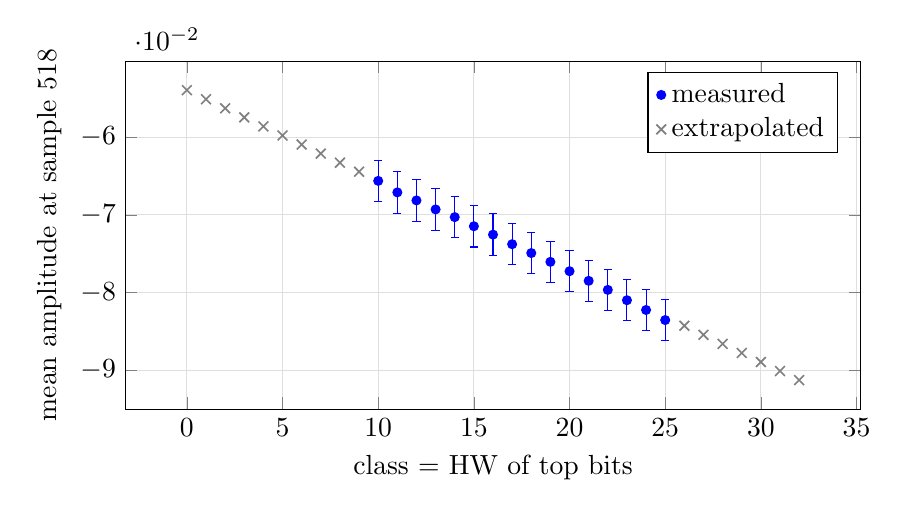
\begin{tikzpicture}
\begin{axis}[
  xlabel={class = HW of top bits},
  ylabel={mean amplitude at sample 518},
  width=0.9\linewidth,
  height=6cm,
  grid=major,
  grid style={gray!25},
  legend pos=north east,
  legend cell align=left,
]
\addplot[blue, semithick, mark=*, mark size=1.5pt, only marks, error bars/.cd, y dir=both, y explicit, error bar style={blue}] coordinates {(10,-0.0656307) +- (0,0.00266584) (11,-0.0671126) +- (0,0.00266584) (12,-0.0681472) +- (0,0.00266584) (13,-0.0693074) +- (0,0.00266584) (14,-0.0702986) +- (0,0.00266584) (15,-0.0714736) +- (0,0.00266584) (16,-0.072553) +- (0,0.00266584) (17,-0.0737876) +- (0,0.00266584) (18,-0.0749251) +- (0,0.00266584) (19,-0.0760602) +- (0,0.00266584) (20,-0.077264) +- (0,0.00266584) (21,-0.0785019) +- (0,0.00266584) (22,-0.0796681) +- (0,0.00266584) (23,-0.0810021) +- (0,0.00266584) (24,-0.0822561) +- (0,0.00266584) (25,-0.0835543) +- (0,0.00266584)};
\addlegendentry{measured}
\addplot[gray, semithick, mark=x, mark size=2.5pt, only marks] coordinates {(0,-0.0539525) (1,-0.0551192) (2,-0.0562859) (3,-0.0574526) (4,-0.0586193) (5,-0.059786) (6,-0.0609527) (7,-0.0621194) (8,-0.0632861) (9,-0.0644528) (26,-0.0842868) (27,-0.0854535) (28,-0.0866202) (29,-0.0877869) (30,-0.0889536) (31,-0.0901203) (32,-0.091287)};
\addlegendentry{extrapolated}
\end{axis}
\end{tikzpicture}
